
\newpage

\begin{flushright}
  \vspace{10cm}
  \rule{18cm}{5pt}
  \rule{18cm}{2pt}\vskip1cm
  \begin{center}
    \begin{bfseries}
      \Huge{\textbf{AWS S3 experiment}}\\
    \end{bfseries}
  \end{center}
  \vspace{1cm}
  \rule{18cm}{2pt}
  \rule{18cm}{5pt}
\end{flushright}
\newpage

\chapter{Procedure followed for the given experiment}
\section{Flowchart}

\begin{figure}[htp]
    \centering
    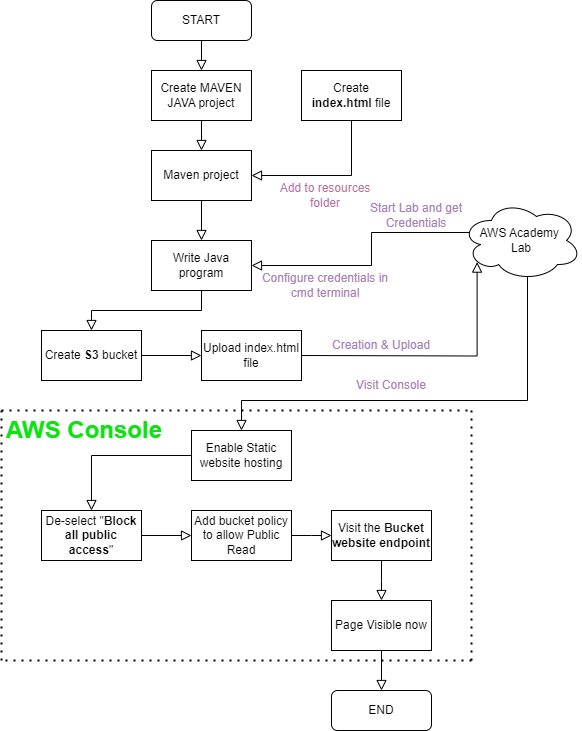
\includegraphics[scale=1, width=12cm,height=15cm]{PROBLEM 2/Flowchart.png}
    \caption{\textbf{\textit{Flowchart describing the operations that I	have performed.}}}
    \label{fig:flowchart}
\end{figure}

\section{My overall observation of the Java SDK}
The Java SDK for AWS S3 provides developers with a comprehensive set of tools and APIs for interacting with S3 buckets. It offers extensive documentation and resources, making it easy to understand and utilize the SDK effectively. The SDK supports various operations such as creating, deleting, and managing S3 buckets, as well as uploading, downloading, and manipulating objects within the buckets. It integrates well with other AWS services, allowing developers to build complex applications and workflows. The SDK is optimized for performance, with features like multipart uploads for efficient handling of large files. Overall, the Java SDK for AWS S3 is a powerful and reliable tool for working with S3 buckets in Java applications.

\section{Configurse session credentials}
\begin{itemize}
    \item Open a command terminal \& Enter \textbf{aws configure}
    \item Enter the Access key ID \& Secret access  key (found in the details section of AWS academy, after Starting the lab)
    \item This will create and configure the credentials file inside  
 the folder \newline \textbf{\path{C:\Users\<your_name>\.aws}}
\end{itemize}
\section{Maven project creation}
\begin{itemize}
  \item A maven Java project was created
  \item Following AWS dependencies were added to the \textit{pom.xml} file:
        \begin{itemize}
          \item SDK:
                \lstdefinelanguage{XML}
                {
                  morestring=[b]",
                  morestring=[s]{>}{<},
                  morecomment=[s]{<?}{?>},
                  stringstyle=\color{blue},
                  identifierstyle=\color{magenta},
                  keywordstyle=\color{cyan},
                  morekeywords={dependency, groupId, artifactId, version, type, scope}
                }

                \lstset{
                  language=XML,
                  basicstyle=\ttfamily,
                  numbers=left,
                  numberstyle=\small\ttfamily\color{gray},
                  showstringspaces=false,
                  breaklines=true,
                  frame=single,
                  backgroundcolor=\color{gray!10},
                  captionpos=b,
                  escapeinside={(*@}{@*)}  % To escape to LaTeX within code
                }


                \begin{lstlisting}
<dependencies>
    <dependency>
        <groupId>software.amazon.awssdk</groupId>
        <artifactId>bom</artifactId>
        <version>2.2.0</version>
        <type>pom</type>
        <scope>import</scope>
    </dependency>
</dependencies>
\end{lstlisting}

        \end{itemize}
        \begin{itemize}
          \item S3:
                \lstdefinelanguage{XML}
                {
                  morestring=[b]",
                  morestring=[s]{>}{<},
                  morecomment=[s]{<?}{?>},
                  stringstyle=\color{blue},
                  identifierstyle=\color{magenta},
                  keywordstyle=\color{cyan},
                  morekeywords={dependency, groupId, artifactId, version, type, scope}
                }

                \lstset{
                  language=XML,
                  basicstyle=\ttfamily,
                  numbers=left,
                  numberstyle=\small\ttfamily\color{gray},
                  showstringspaces=false,
                  breaklines=true,
                  frame=single,
                  backgroundcolor=\color{gray!10},
                  captionpos=b,
                  escapeinside={(*@}{@*)}  % To escape to LaTeX within code
                }
                \begin{lstlisting}
<dependency>
    <groupId>software.amazon.awssdk</groupId>
    <artifactId>s3</artifactId>
    <version>2.2.0</version>
</dependency>
\end{lstlisting}

        \end{itemize}

\end{itemize}
\newpage
\section{Creation of Index.html file}
\begin{itemize}
  \item A \textit{index.html} file was created inside the \textit{resources }folder of the \textbf{maven project}
        \newline\newline
        index.html:
        \lstset{
          language=HTML,
          basicstyle=\ttfamily,
          keywordstyle=\color{blue},
          commentstyle=\color{green!60!black},
          stringstyle=\color{red},
          numbers=left,
          numberstyle=\small\ttfamily\color{gray},
          showstringspaces=false,
          breaklines=true,
          frame=single,
          backgroundcolor=\color{gray!10},
          captionpos=b,
          escapeinside={(*@}{@*)}  % To escape to LaTeX within code
        }

        \begin{lstlisting}
<!DOCTYPE html>
<html>
<head>
    <title>My Profile</title>
</head>
<body>
<h1>My Profile Information</h1>
<p>
    <strong>Name:</strong> Vikram Venkatapathi<br>
    <strong>Banner Number:</strong> B00936916<br>
    <strong>Email:</strong> vk485591@dal.ca<br>
</p>
<p>
    <em>This assignment is my own work; I did not take help from anyone.</em>
</p>
</body>
</html>
\end{lstlisting}
\end{itemize}

\section{Java program to create S3 Bucket}
\begin{itemize}
  \item A Java program was written using the AWS SDK  to
        \begin{itemize}
          \item use the session specific ACCESS\_KEY\_ID \& SECRET\_ACCESS\_KEY
          \item create an S3 bucket following the naming conventions (Bucket name : b00936916-a1)
          \item upload the index.html file to the created bucket.
        \end{itemize}
  \item Comments were added following the Java Docs specification (Refer \ref{fig:javaDocs})
        \begin{figure}[htp]
          \centering
          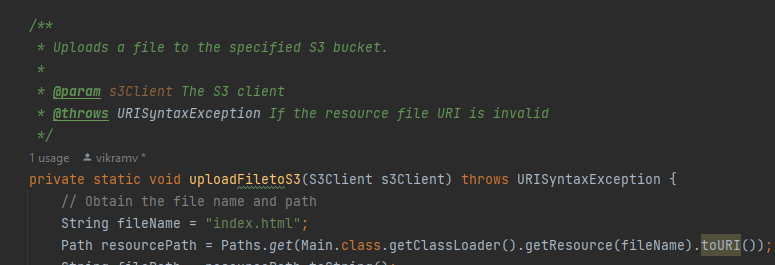
\includegraphics[scale=1, width=10cm,height=3cm]{PROBLEM 2/Snaps/1. Java docs specs.png}
          \caption{\textbf{\textit{Comments added, based on Java Docs specification}}}
          \label{fig:javaDocs}
        \end{figure}
    \item Main.java
   
\lstset{
tabsize = 4, %% set tab space width
showstringspaces = false, %% prevent space marking in strings, string is defined as the text that is generally printed directly to the console
numbers = left, %% display line numbers on the left
commentstyle = \color{green}, %% set comment color
keywordstyle = \color{blue}, %% set keyword color
stringstyle = \color{red}, %% set string color
rulecolor = \color{black}, %% set frame color to avoid being affected by text color
basicstyle = \small \ttfamily , %% set listing font and size
breaklines = true, %% enable line breaking
numberstyle = \tiny,
}

\begin{lstlisting}[language = Java , frame = trBL , firstnumber = last , escapeinside={(*@}{@*)}]
package org.example;

import software.amazon.awssdk.auth.credentials.ProfileCredentialsProvider;
import software.amazon.awssdk.core.sync.RequestBody;
import software.amazon.awssdk.regions.Region;
import software.amazon.awssdk.services.s3.S3Client;
import software.amazon.awssdk.services.s3.model.CreateBucketRequest;
import software.amazon.awssdk.services.s3.model.CreateBucketResponse;
import software.amazon.awssdk.services.s3.model.PutObjectRequest;
import software.amazon.awssdk.services.s3.model.S3Exception;

import java.io.File;
import java.net.URISyntaxException;
import java.nio.file.Path;
import java.nio.file.Paths;

public class Main {
    private static String bucketName = "b00936916-a1";
    private static String region = "us-east-1";

    /**
     * Main method to create an S3 bucket and upload a file to it.
     *
     * @param args Command-line arguments
     * @throws URISyntaxException If the file path is not a valid URI
     */
    public static void main(String[] args) throws URISyntaxException {
        // Create the credentials provider
        //Retrieve the AWS Access Key ID & AWS Secret Access Key from ./aws/credentials file
        ProfileCredentialsProvider credentialsProvider = ProfileCredentialsProvider.create();

        // Create the S3 client
        S3Client s3Client = S3Client.builder()
                .region(Region.of(region))
                .credentialsProvider(credentialsProvider)
                .build();

        // Call the method to create an S3 bucket
        createS3Bucket(s3Client);

        // Call the method to upload a file to S3
        uploadFiletoS3(s3Client);
    }

    /**
     * Creates an S3 bucket with the specified bucket name.
     *
     * @param s3Client The S3 client
     */
    private static void createS3Bucket(S3Client s3Client) {
        try {
            // Create a request to create an S3 bucket with the specified bucket name
            CreateBucketRequest createBucketRequest = CreateBucketRequest.builder()
                    .bucket(bucketName)
                    .build();

            // Send the create bucket request to the S3 service
            CreateBucketResponse createBucketResponse = s3Client.createBucket(createBucketRequest);
        } catch (S3Exception e) {
            if (e.awsErrorDetails().errorCode().equals("BucketAlreadyExists")) {
                System.err.print("Failed to create bucket. Bucket name already exists");
            }
        }
    }

    /**
     * Uploads a file to the S3 bucket.
     *
     * @param s3Client The S3 client
     * @throws URISyntaxException If the file path is not a valid URI
     */
    private static void uploadFiletoS3(S3Client s3Client) throws URISyntaxException {
        // Obtain the file name and path
        String fileName = "index.html";
        Path resourcePath = Paths.get(Main.class.getClassLoader().getResource(fileName).toURI());
        String filePath = resourcePath.toString();

        // Create a request to put the object in the S3 bucket
        PutObjectRequest putObjectRequest = PutObjectRequest.builder()
                .bucket(bucketName)
                .key(filePath)
                .build();

        // Upload the file to S3
        s3Client.putObject(putObjectRequest, RequestBody.fromFile(new File(filePath)));
    }
}

/** References : 
* Code snippets were referred from official AWS SDK documentation:

@see <a href="https://docs.aws.amazon.com/sdk-for-java/latest/developer-guide/examples-s3-buckets.html ">Create S3 bucket</a>
@see <a href="https://docs.aws.amazon.com/sdk-for-java/latest/developer-guide/examples-s3-objects.html">PUT object in S3 bucket</a>
*/
\end{lstlisting}
    
\end{itemize}

\section{Operations on the AWS console}

\begin{enumerate}
  \item Goto S3 Service
  \item Select \textbf{Buckets}, in the left-hand side menu
  \item Goto \textbf{Permissions} section
  \item Scroll down, Edit \textbf{Static website hosting}
        \begin{enumerate}
          \item Select \textbf{Enable}
          \item Specify the uploaded index file name in the \textbf{Index document} text box
          \item Click \textbf{Save changes}
        \end{enumerate}
  \item Go to the created bucket
        \begin{enumerate}
          \item Go to the \textbf{Properties} section
          \item Scroll to the end, till "Static website hosting". 
          \item Visit the \textbf{Bucket website endpoint}
          \item \textbf{Access Denied} - because the bucket is  \textbf{not Public}, and doesn't allow \textbf{Public Read Access}
        \end{enumerate}
  \item Go to the created Bucket
        \begin{enumerate}
            \item Go to \textbf{Permissions} section
            \item De-select \textbf{Block all public access}
          \item Go to the \textbf{Bucket policy} section, \textbf{Edit} it
          \item Add the following policy and \textbf{Save changes}
           \newpage
                \lstdefinelanguage{XML}
                {
                  morestring=[b]",
                  morestring=[s]{>}{<},
                  morecomment=[s]{<?}{?>},
                  stringstyle=\color{blue},
                  identifierstyle=\color{magenta},
                  keywordstyle=\color{cyan},
                  morekeywords={dependency, groupId, artifactId, version, type, scope}
                }

                \lstset{
                  language=XML,
                  basicstyle=\ttfamily,
                  numbers=left,
                  numberstyle=\small\ttfamily\color{gray},
                  showstringspaces=false,
                  breaklines=true,
                  frame=single,
                  backgroundcolor=\color{gray!10},
                  captionpos=b,
                  escapeinside={(*@}{@*)}  % To escape to LaTeX within code
                }


                \begin{lstlisting}
{
    "Version": "2012-10-17",
    "Statement": [
        {
            "Sid": "PublicReadGetObject",
            "Effect": "Allow",
            "Principal": "*",
            "Action": "s3:GetObject",
            "Resource": "arn:aws:s3:::b00936916-a1/*"
        }
    ]
}

\end{lstlisting}

        \end{enumerate}
        % \newpage
        \item Go visit the website endpoint, Hit Refresh
        \item You can view the index.html file now. 
        
\end{enumerate}
\textbf{ NOTE: Refer to the following Screenshots for the steps mentioned above.
}\chapter{Screenshots}

\begin{figure}[htp]
    \centering
    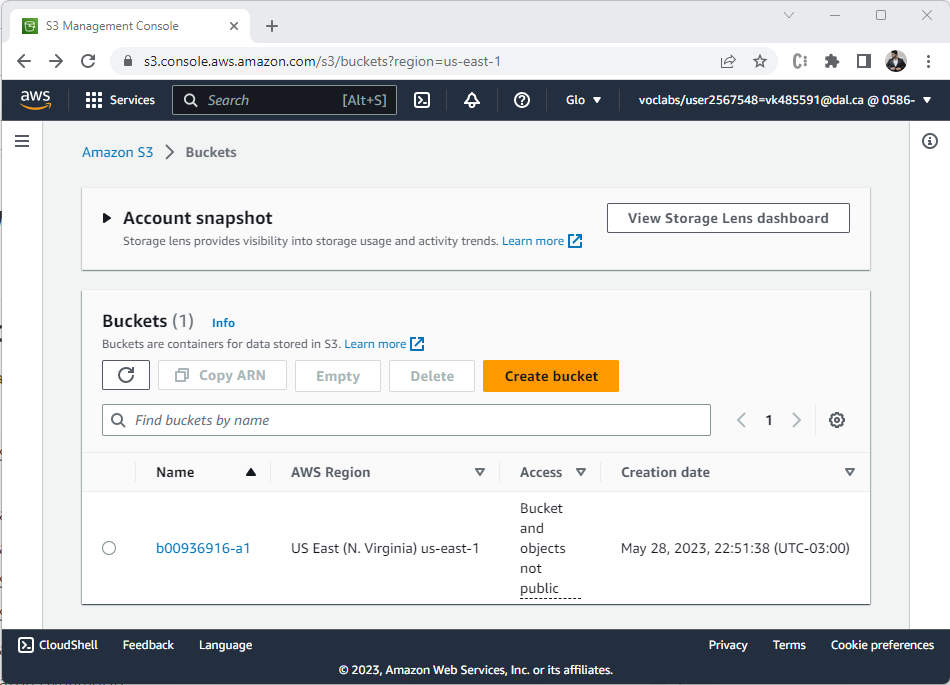
\includegraphics[scale=1, width=15cm,height=7cm]{PROBLEM 2/Snaps/2. Bucket created.png}
    \caption{\textbf{\textit{Bucket created}}}
    \label{fig:bucket_created}
\end{figure}

\begin{figure}[htp]
    \centering
    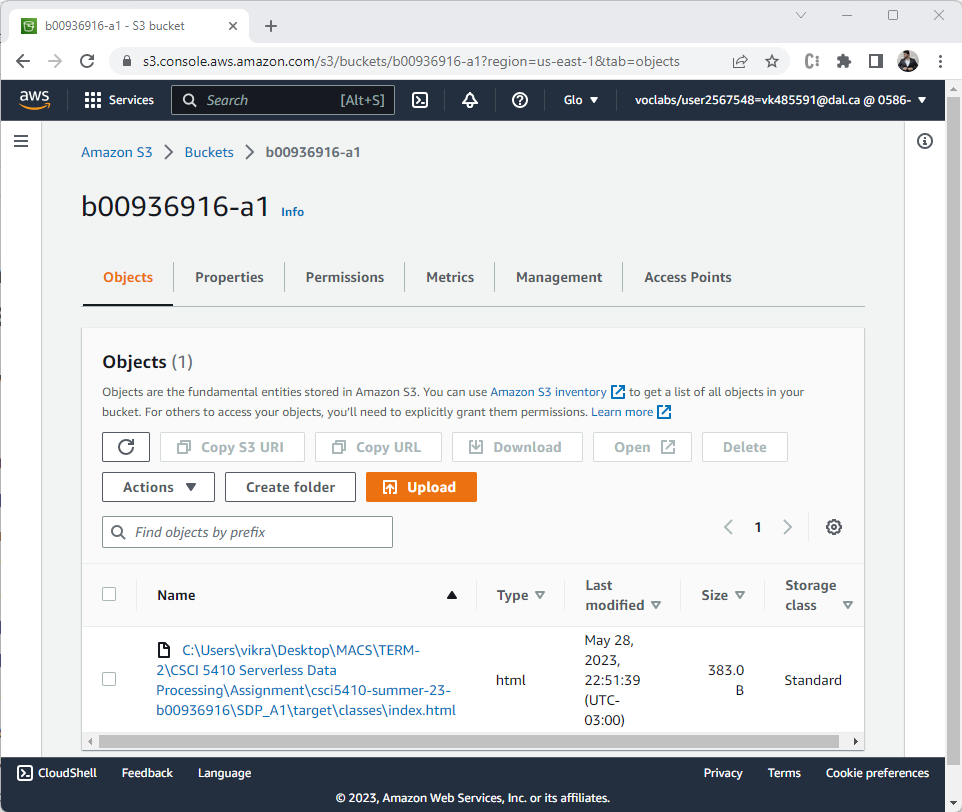
\includegraphics[scale=1, width=15cm,height=7.5cm]{PROBLEM 2/Snaps/3. File uploaded.png}
    \caption{\textbf{\textit{Index.html file uploaded }}}
    \label{fig:index_file_uploaded}
\end{figure}

\begin{figure}[htp]
    \centering
    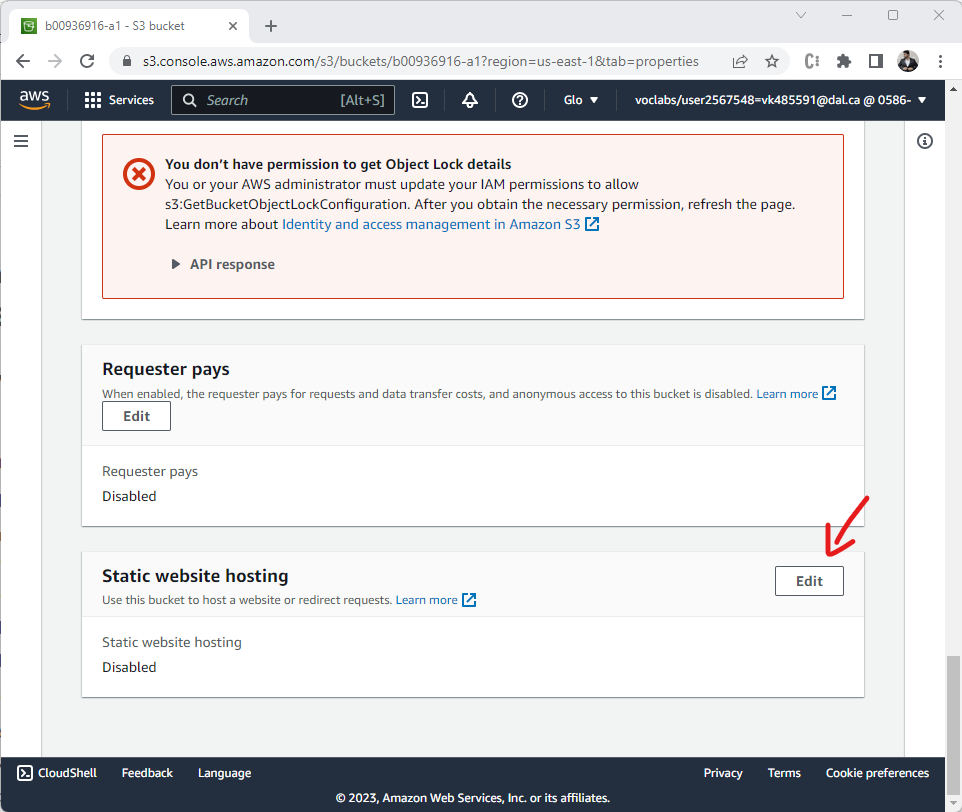
\includegraphics[scale=1, width=15cm,height=7.5cm]{PROBLEM 2/Snaps/4. Goto Properties-Enable website hosting.png}
    \caption{\textbf{\textit{Enable website hosting}}}
    \label{fig:enable_hosting}
\end{figure}

\begin{figure}[htp]
    \centering
    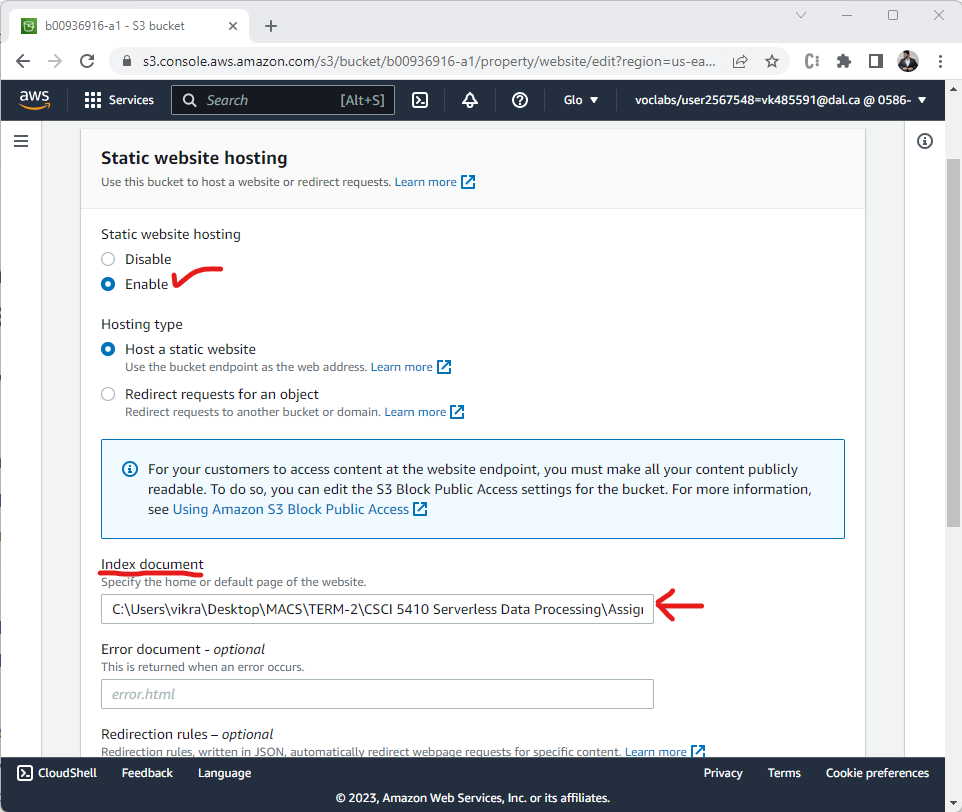
\includegraphics[scale=1, width=15cm,height=7.5cm]{PROBLEM 2/Snaps/5. Specify index.html file.png}
    \caption{\textbf{\textit{Specify the index.html file name to host the website }}}
    \label{fig:Specify_index_file}
\end{figure}

\begin{figure}[htp]
    \centering
    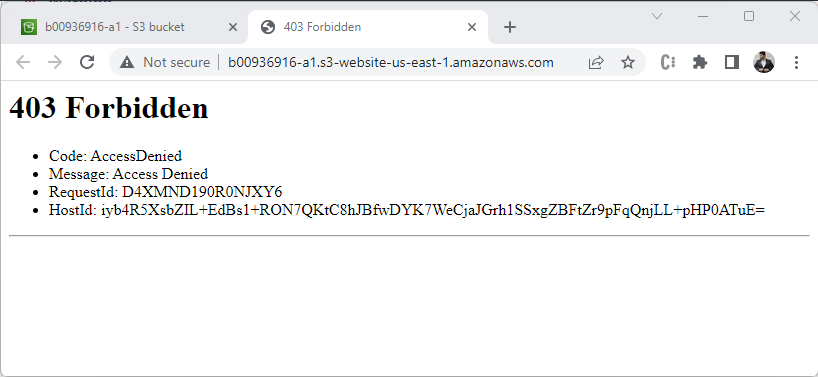
\includegraphics[scale=1, width=15cm,height=7.5cm]{PROBLEM 2/Snaps/6. Access denied.png}
    \caption{\textbf{\textit{Access is denied since bucket is not public and doesn't allow READ access }}}
    \label{fig:access_denied}
\end{figure}

\begin{figure}[htp]
    \centering
    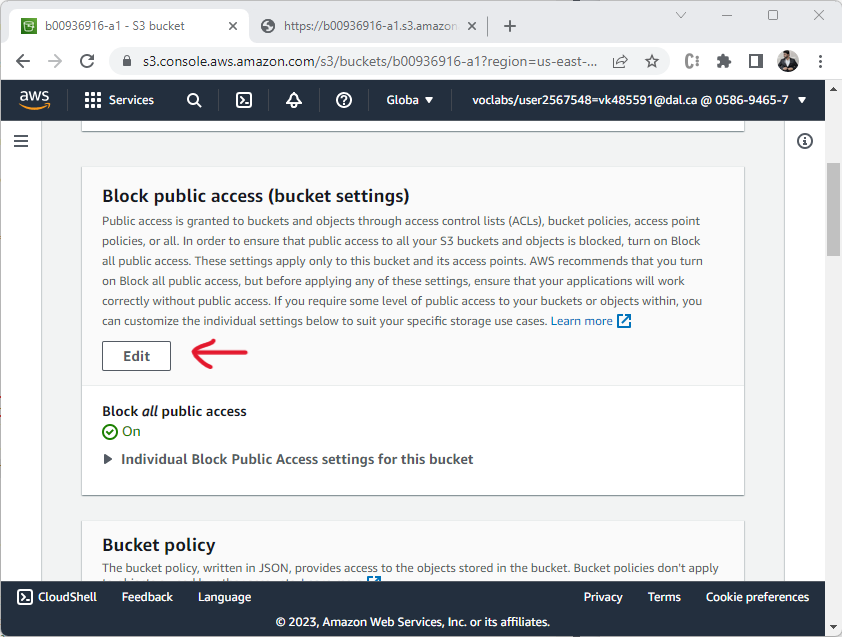
\includegraphics[scale=1, width=15cm,height=7.5cm]{PROBLEM 2/Snaps/7. Edit block public access.png}
    \caption{\textbf{\textit{ Edit block all public access}}}
    \label{fig:edit_block}
\end{figure}

\begin{figure}[htp]
    \centering
    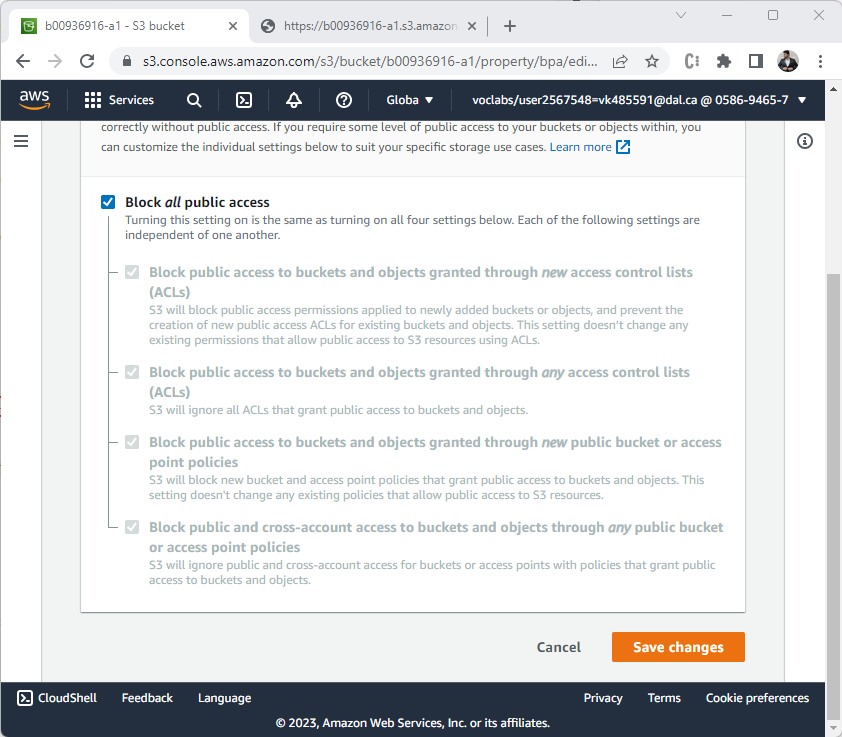
\includegraphics[scale=1, width=15cm,height=7.5cm]{PROBLEM 2/Snaps/8.1 De-select Block all public access.png}
    \caption{\textbf{\textit{De-select Bloack all public access }}}
    \label{fig:deselect_block}
\end{figure}

\begin{figure}[htp]
    \centering
    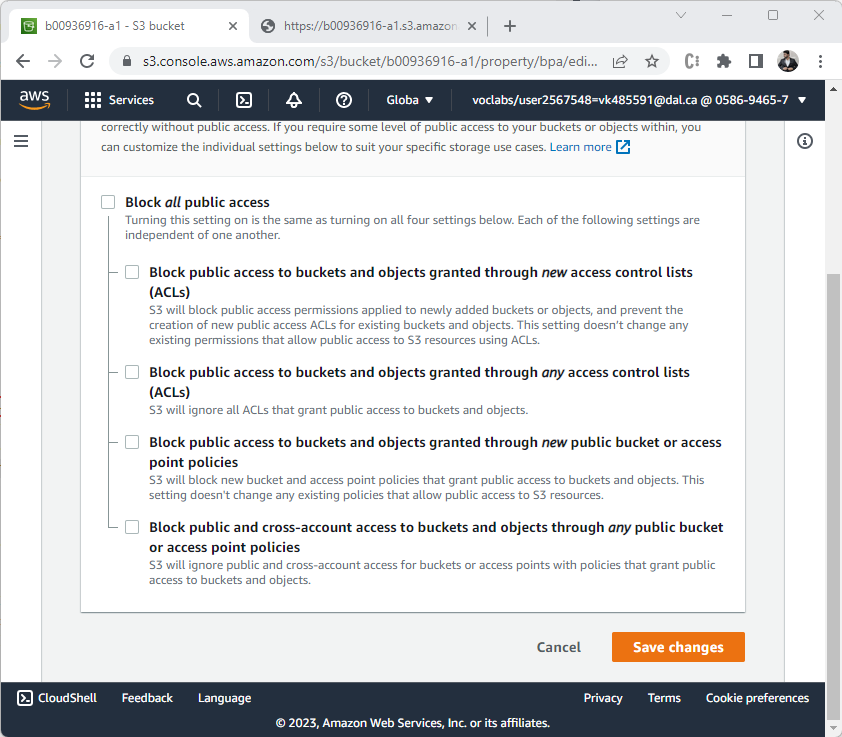
\includegraphics[scale=1, width=15cm,height=7.5cm]{PROBLEM 2/Snaps/8.2 De-selected.png}
    \caption{\textbf{\textit{De-selected}}}
    \label{fig:after_deselect}
\end{figure}

\begin{figure}[htp]
    \centering
    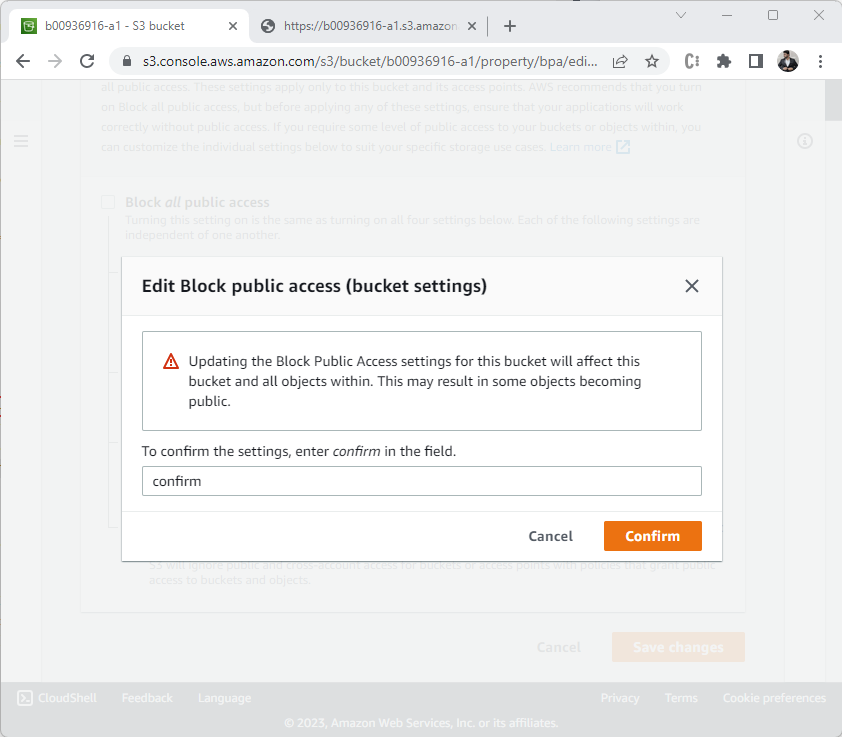
\includegraphics[scale=1, width=15cm,height=7.5cm]{PROBLEM 2/Snaps/8.3 Confirm it.png}
    \caption{\textbf{\textit{ Confirm the action}}}
    \label{fig:confirm_deselect}
\end{figure}

\begin{figure}[htp]
    \centering
    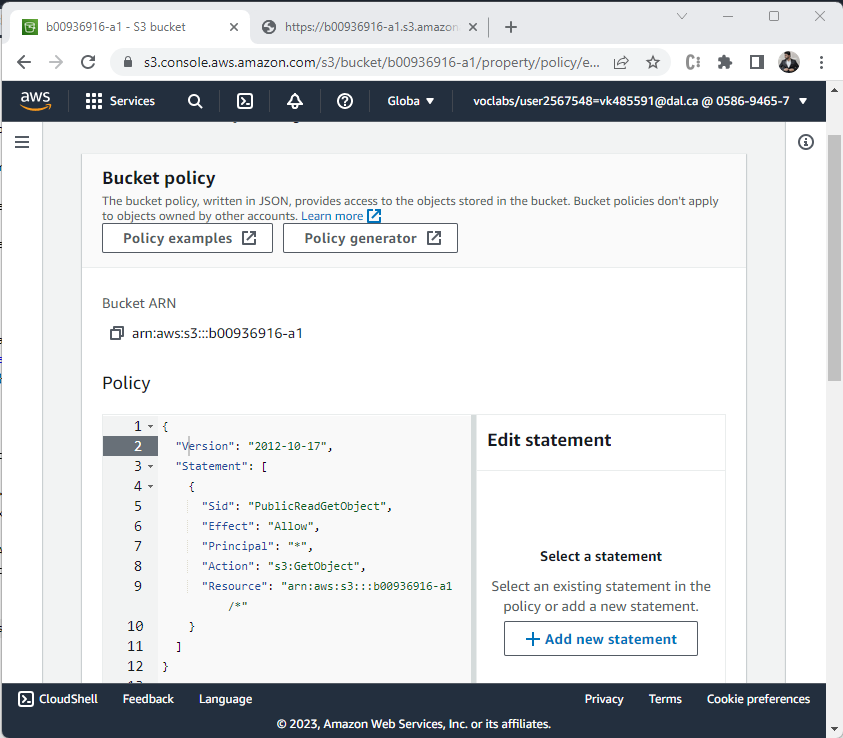
\includegraphics[scale=1, width=15cm,height=7.5cm]{PROBLEM 2/Snaps/9. Edit bucket policy.png}
    \caption{\textbf{\textit{Add bucket policy }}}
    \label{fig:edit_policy}
\end{figure}

\begin{figure}[htp]
    \centering
    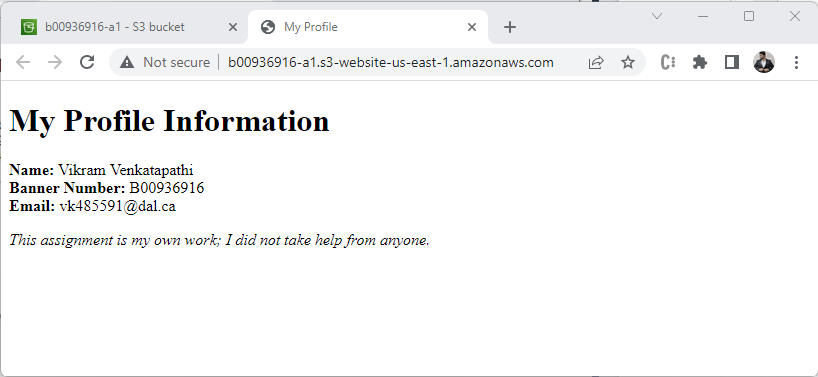
\includegraphics[scale=1, width=15cm,height=7.5cm]{PROBLEM 2/Snaps/10. Refresh browser - page visible now.png}
    \caption{\textbf{\textit{Refresh the browser - Page is now visible }}}
    \label{fig:refresh_browser}
\end{figure}

\begin{figure}[htp]
    \centering
    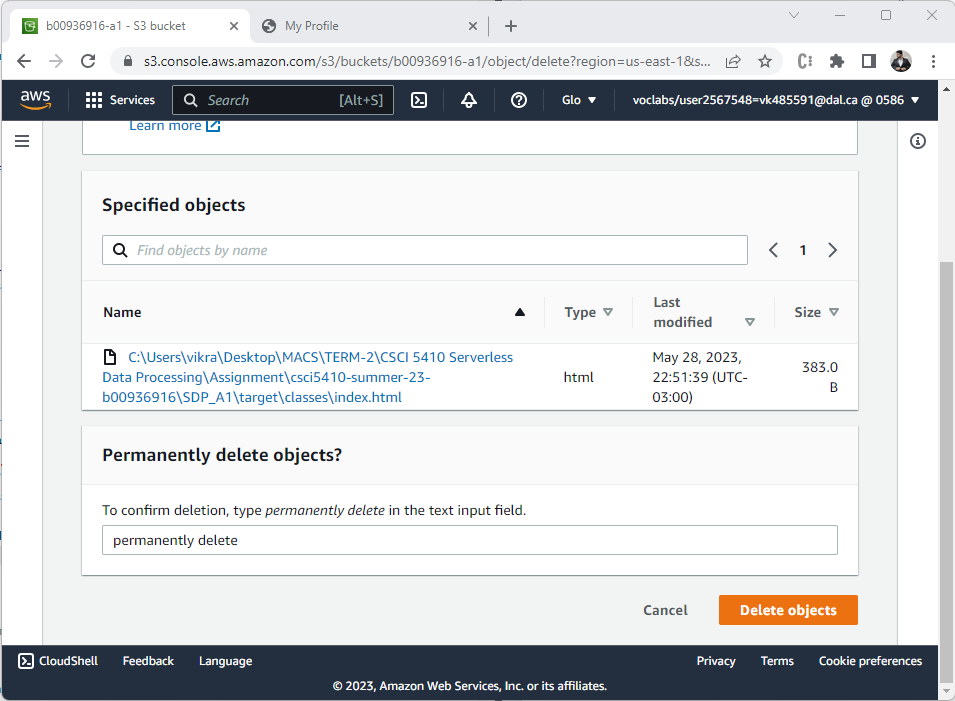
\includegraphics[scale=1, width=15cm,height=7.5cm]{PROBLEM 2/Snaps/11. Empty Bucket.png}
    \caption{\textbf{\textit{ Empty the bucket, after all tasks are done}}}
    \label{fig:empty_bucket}
\end{figure}

\begin{figure}[htp]
    \centering
    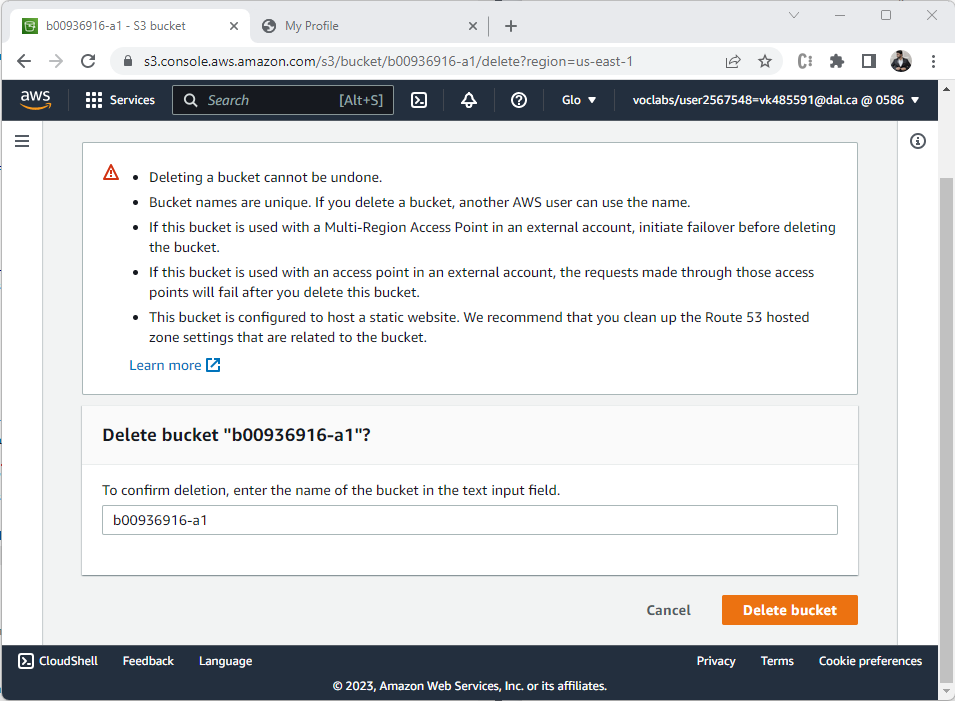
\includegraphics[scale=1, width=15cm,height=7.5cm]{PROBLEM 2/Snaps/12. Delete bucket.png}
    \caption{\textbf{\textit{ Delete the bucket, Save resources and credits}}}
    \label{fig:delete_bucket}
\end{figure}


\newpage